% Chapter Template
\chapter{CNN: implementazione e addestramento} % Main chapter title
\label{Capitolo4}
\def \path	 {Figures/C4}
In questo capitolo verranno messi in pratica i concetti introdotti nel Capitolo \ref{Capitolo3}. In particolare, verrà addestrata una CNN su 2 dataset, MNIST e CIFAR. I risultati serviranno da confronto con ResNet, la rete utilizzata nel Capitolo 5. 
%--------------------------------------------------------------------
%	SECTION 1
%--------------------------------------------------------------------
\section{Modello di CNN basato su LeNet}
La rete implementata è basata sulla capostipite delle CNN, \texttt{LeNet5}, resa celebre da Y. LeCun per il riconoscimento di caratteri, anche scritti a mano\parencite{lenet}.  L'architettura è rappresentata in figura \ref{fig:lenet}. Si noti che la rete è appositamente progettata per avere in input immagini di 32x32 pixel, adatta ai dataset che si introduranno dopo. 
\begin{figure}[h!]
 \centering
 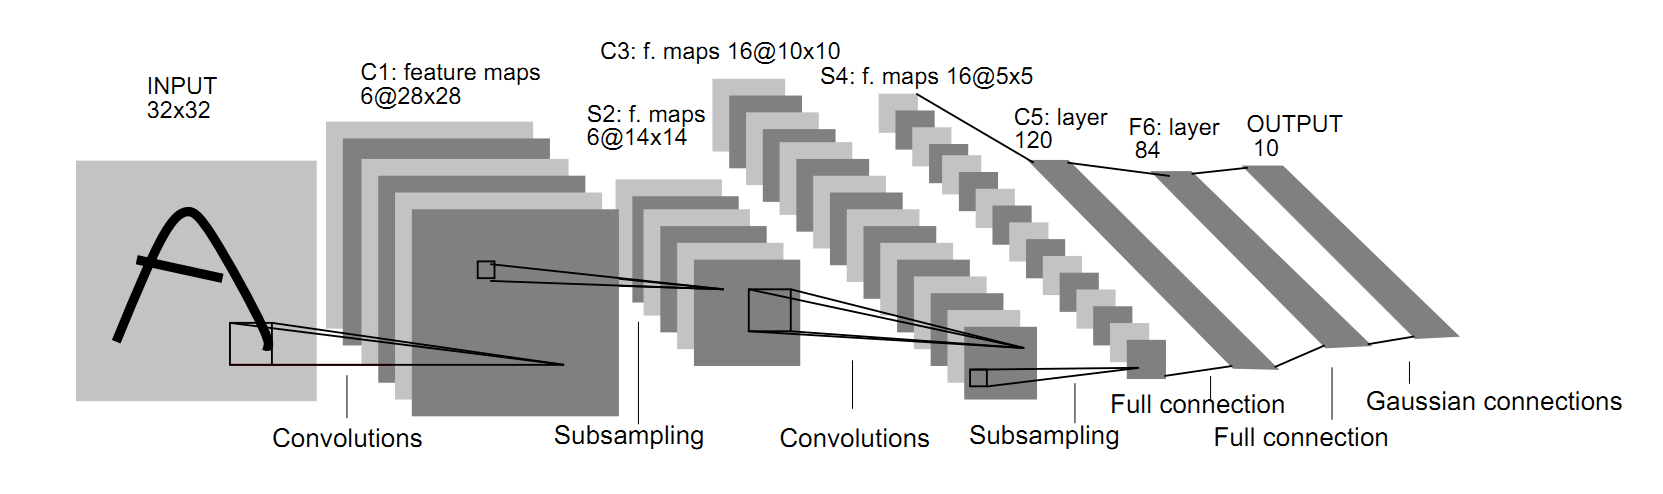
\includegraphics[width=1.0\textwidth]{\path/lenet.png} 
 \caption{Architettura di LeNet5, qui per il riconoscimento di caratteri scritti a mano}
 \label{fig:lenet}
\end{figure}	\\
Per implementare la rete verrà impiegato il già citato framework Torch. Per saperne di più su Torch e sugli utilizzi basilari per le reti neurali si veda l'appendice \ref{AppendixB}.

Si procede quindi, ad implementare la rete costituita da: 
\begin{itemize}
\item 2x $\rightarrow$ Convolutional layers - ReLU - Pooling layers
\item 1x $\rightarrow$ Multi-layer perceptron completamente connesso, con 1 hidden layer 
\end{itemize}

%% inserire codice rete %% 

\subsection{Definire la loss function}
Ora che si ha un modello, va definita una funzione di costo da minimizzare che, come visto nel capitolo 2, sta alla base dell’apprendimento. Nel capitolo 2 però, si era definito tutto "a mano", mentre ora si usano le librerie di Torch. \\Con Torch si possono definire diverse funzioni di costo, a seconda del principio di apprendimento che vogliamo utilizzare. Come ad esempio lo scarto quadratico che però non è in generale una scelta ottimale. Una delle più convienienti per i problemi di classificazione è la \emph{negative-likelihood} (likelihood = funzione di verosimiglianza). La negative-likelihood necessita in ingresso di un vettori di probabilità logaritmiche normalizzate. Quindi, prima si trasforma l’output del classificatore in probabilità logaritmica aggiungendo un modulo chiamato \texttt{LogSoftMax} e poi si calcola l'errore sulla negative-likelihood. In Torch questo è semplicissimo: 

\begin{lstlisting}[language={[5.2]Lua}]
--add a Log-SoftMax classifier at the end of the Net
model:add(nn.LogSoftMax())

--criterion (i.e. the loss) will be the negative-likelihood
criterion = nn.ClassNLLCriterion()
\end{lstlisting}

\section{}


%--------------------------------------------------------------------
%	SECTION 2
%--------------------------------------------------------------------
\section{MNIST}
MNIST è un dataset di cifre scritte a mano, disponibile sul sito di Y. LeCun, costituito da un training set di 60000 esempi e un test set di 10000. Le immagini sono già state normalizzate e sono croppate in modo da avere la cifra esattamente al centro dell’immagine, e per questo richiedono un pre-processing praticamente nullo.
Quindi, utilizzando il codice della sezione precedente e lanciando un addestramento su MNIST si avranno i risultati in 
%% altri metodi però fanno fatica %% 

%--------------------------------------------------------------------
%	SECTION 3
%--------------------------------------------------------------------
\section{CIFAR: preprocessing}
MNIST è uno dei dataset più semplici in circolazione
%--------------------------------------------------------------------
%	SECTION 4
%--------------------------------------------------------------------
\section{CIFAR: addestramento}


Vedremo nel capitolo seguente un confronto dei risultati di una CNN con un'archittettura allo stato dell'arte testata sullo stesso dataset. 



\begin{figure}[h!]
 \centering
 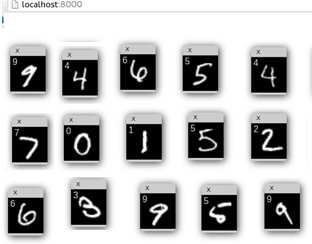
\includegraphics[width=1.0\textwidth]{\path/mnist-screen.png} 
 \caption{Esempi di cifre classificate correttamente}
 \label{fig:mnist-correct}
\end{figure}

\begin{figure}[h!]
 \centering
 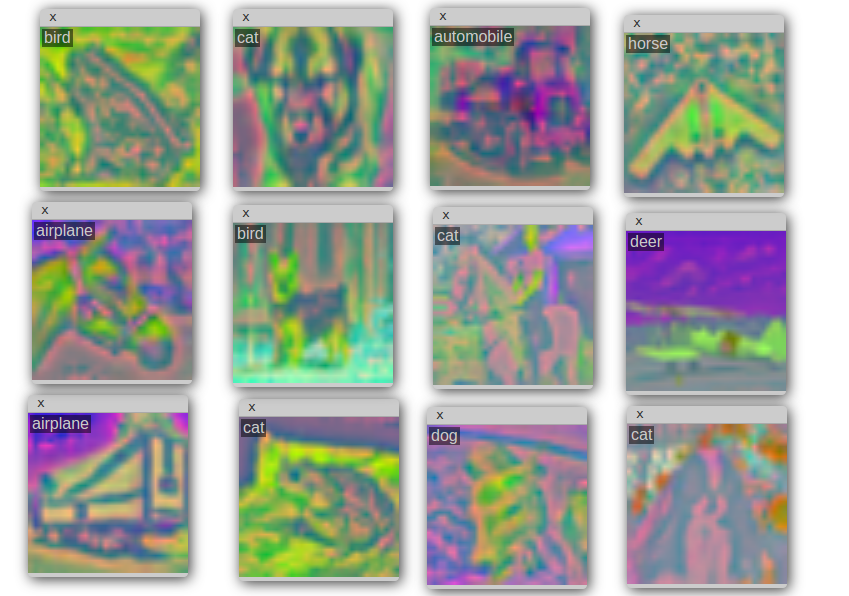
\includegraphics[width=1.0\textwidth]{\path/cifar-wrong.png} 
 \caption{Esempi di animali classificati erroneamente}
 \label{fig:cifar-wrong}
\end{figure}

\begin{figure}[h!]
 \centering
 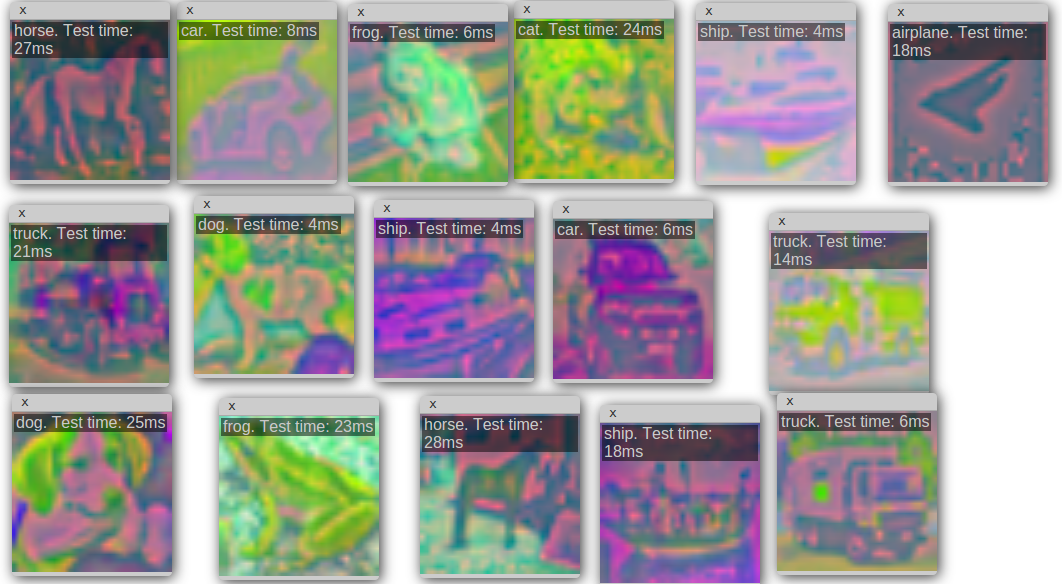
\includegraphics[width=1.0\textwidth]{\path/cifar-correct.png} 
 \caption{Esempi di animali classificati correttamente}
 \label{fig:cifar-correct}
\end{figure}

\begin{figure}[h!]
 \centering
 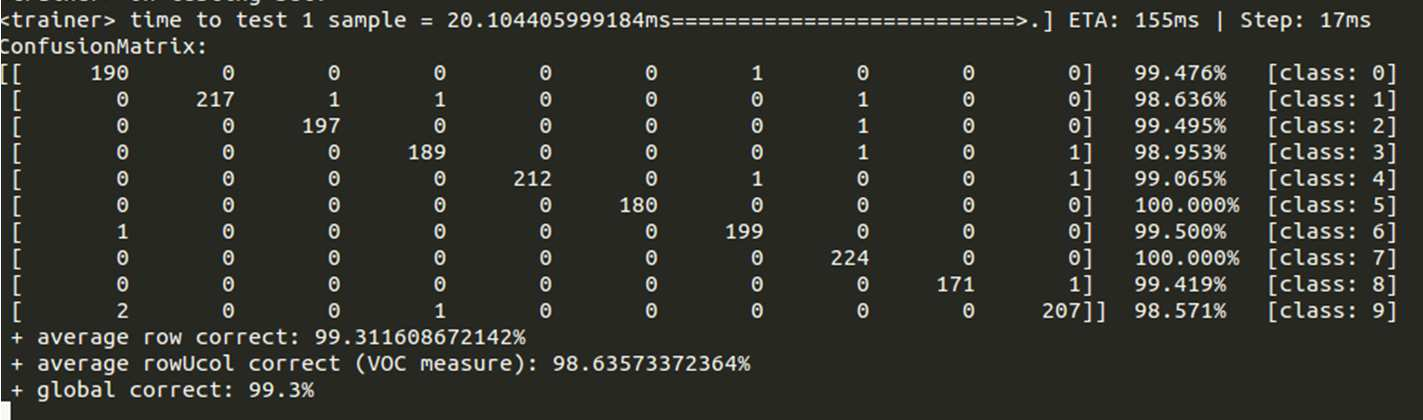
\includegraphics[width=1.0\textwidth]{\path/mnist-training.png} 
 \caption{Confusion Matrix MNIST: la matrice che mostra le percentuali di accuratezza ed errore sul validation set per ogni classe}
 \label{fig:mnist-training}
\end{figure}

\begin{figure}[h!]
 \centering
 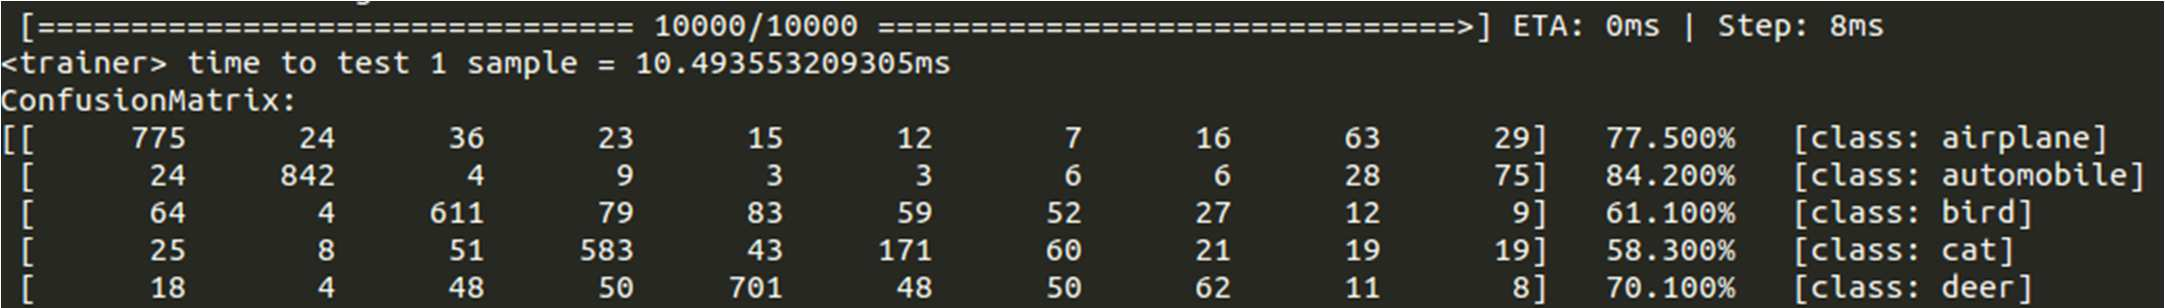
\includegraphics[width=1.0\textwidth]{\path/cifar-train.png} 
 \caption{Confusion Matrix CIFAR: la matrice che mostra le percentuali di accuratezza ed errore sul validation set per ogni classe}
 \label{fig:cifar-training}
\end{figure}

\begin{figure}
\centering
\begin{subfigure}{.5\textwidth}
  \centering
 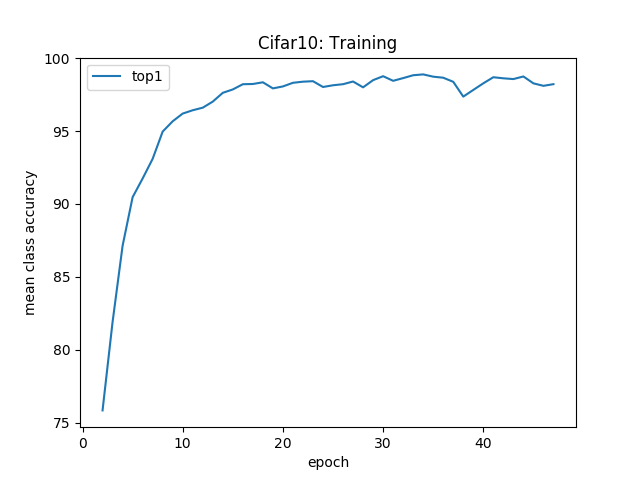
\includegraphics[width=1\textwidth]{\path/training.png} 
  \caption{Accuracy sul training set}
 \label{fig:training}
\end{subfigure}%
\begin{subfigure}{.5\textwidth}
  \centering
 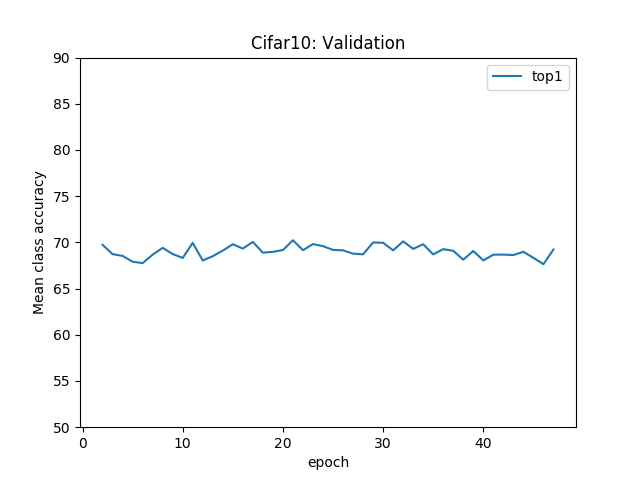
\includegraphics[width=1\textwidth]{\path/validation.png} 
  \caption{Accuracy sul validation set}
 \label{fig:validation}
\end{subfigure}
\caption{Performance della rete in training e validation}
\label{fig:subfigure}
\end{figure}
